
% ----------------------------------------------------------
% CAPÍTULO 03 - METODOLOGIA E DADOS
% ----------------------------------------------------------

\chapter{Metodologia e dados} \label{cha:metodologia}

Este capítulo descreve os modelos de Equilíbrio Geral Computável e microssimulação comportamental utilizados para estimar os efeitos do comércio internacional sobre a distribuição da renda familiar e os níveis de pobreza no Brasil. Também se apresenta a base de dados usada para a calibragem dos referidos modelos e a implementação da estratégia empírica para simular os efeitos de um choque de liberalização comercial, além de apresentar as ferramentas utilizadas para calcular os índices desigualdade de renda e pobreza.


\section{O modelo de Equilíbrio Geral Computável} \label{sec:egc}

Utiliza-se o modelo nacional estático de Equilíbrio Geral Computável para o Brasil, o ORANIG-BR, adaptado para cumprir os objetivos propostos nesta dissertação. Esse modelo partiu da estrutura teórica do ORANI \cite{dixit80}, de tradição australiana do tipo Johansen\footnote{Caracteriza-se por ter um escopo matemático concebido a partir de um conjunto de equações linearizadas e as soluções são apresentadas como elasticidades, representando as taxas de crescimento, sendo possível diversos tipos de fechamento.}.

Sua especificação teórica é composta por blocos de equações que determinam as relações de oferta a partir das hipóteses de otimização e \textit{market clearing}. O modelo incorpora os pressupostos neoclássicos das firmas minimizadoras de custos, famílias maximizadoras de utilidade e equilíbrio dos mercados - esta sendo garantida desde que a oferta e demanda se igualem para o mercado de produtos e serviços domésticos, importados, margens e para o mercado de trabalho.

O uso do modelo de EGC para estudos de análise política, sobretudo sobre impactos e efeitos de algum determinado fenômeno econômico, político ou histórico se tornou cada vez mais frequente na literatura econômica. Há diversos benefícios em trabalhar com esse modelo: é possível operar com altos níveis de desagregação setorial e regional; considerar as relações de interdependência entre os setores e os agentes econômicos; e capturar o efeito-renda e efeito-preço, que estão diretamente relacionados com os canais de transmissão entre comércio internacional e desigualdade de renda e pobreza \cite{anderson20}.

Para esta dissertação, foram realizadas três principais modificações no modelo ORANIG-BR: 1- o fator trabalho foi dividido em três categorias que refletem os diferentes tipos de força de trabalho a partir do nível de escolaridade; 2- as famílias foram divididas em cem categorias de acordo com a renda; e 3- o fluxo das exportações foi dividido entre vinte e seis parceiros comerciais. A Figura~\ref{fig:estrutura_orani} apresenta a estrutura esquemática do modelo ORANIG-BR com as referidas modificações e a Figura~\ref{fig:dados_orani} apresenta a base de dados.


\begin{landscape}
	\begin{figure}
		\centering
		\caption{Representação esquemática do modelo ORANIG-BR} \label{fig:estrutura_orani}
		
\includegraphics[width=0.95\linewidth]{Imagens/002.ai}
		\footnotesize \\
		Fonte: elaboração própria (2024) a partir de \textcite{souza15}
	\end{figure}
\end{landscape}

\begin{figure}[H]
	\centering
	\caption{Base de dados do modelo ORANIG-BR} \label{fig:dados_orani}
	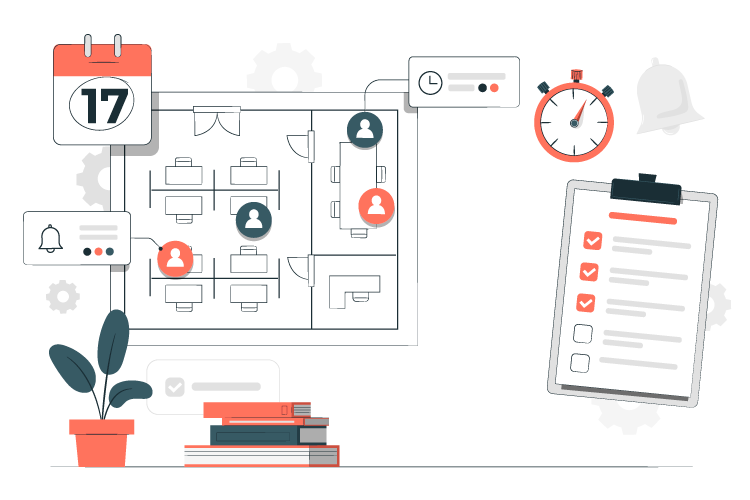
\includegraphics[width=\textwidth]{Imagens/003.ai}
	\footnotesize
	Fonte: elaboração própria (2024) a partir de \textcite{horridge00}
\end{figure}


\subsection{Produção} \label{subsec:producao}

Os setores produtivos seguem os pressupostos neoclássicos de minimização dos custos numa estrutura de mercado de concorrência perfeita, sujeitos a tecnologias de retornos constantes de escala - representadas por funções CES e Leontief. A Figura \ref{fig:estrutura_producao} apresenta a estrutura de produção do modelo. Há cerca de três produtos: 1- bens intermediários; 2- fatores primários; e 3- outros fatores\footnote{"Outros fatores" são as taxas e subsídios do modelo.}. Para se produzir o primeiro, deve-se combinar uma determinada composição das \textit{commodities} disponíveis, decidindo sua origem - se doméstico ou importado. Para produzir o segundo, deve-se combinar quantidades relativas de capital e trabalho, sendo que este é determinado a partir de uma combinação dos três tipos disponíveis de trabalhadores.

Desse modo, para poder produzir nesse modelo, deve-se combinar os bens intermediários, os fatores primários e os outros fatores a partir da minimização dos custos da função Leontief\footnote{Isso implica que esses três fatores são complementares perfeitos, não admitindo substituição}.

\begin{align}
	\underset{i = 1, ... , 124}{Leontief} \biggl\{ \frac{X_{ij}}{A_{ij}} \biggr\} = A_jZ_j, \hspace{2cm} j = 1, ... , 65
\end{align}

No qual $X_{ij}$ corresponde ao insumo $i$ da indústria $j$; $Z_j$ é o nível de atividade da indústria $j$; e $A_ij$ é o coeficiente tecnológico. Se este é igual a 1, significa que é o coeficiente insumo-produto que mostra o insumo mínimo efetivo de $i$ necessário para sustentar uma unidade de atividade na indústria $j$ \cite{dixit80}.

A decisão entre a fonte doméstica ou importada é modelada a partir da hipótese de \textcite{armington69} a qual relaciona os insumos de ambas as fontes como substitutos imperfeitos. Desse modo, para capturar esse efeito, assume-se as unidades de um determinado insumo, diferenciáveis apenas pela fonte, são combinadas para fornecer um só insumo, chamado de \textit{insumo efetivo}:

\begin{align}
	X_{ij} = \underset{s = 1, 2}{CES} = \biggl\{ \frac{X_{(is)j}}{A_{(is)j}}; \rho_{ij}, b_{(is)j} \biggl\}, \hspace{2cm} i & = 1, ... , 124 \\ j & = 1, ... , 65 \notag
\end{align}

No qual $X_{(is)j}$ se refere ao insumo $i$ da fonte $s$ pertencente ao setor $j$; $\rho$ e $b$ são parâmetros de substituição entre as variáveis doméstica e importada. 

\begin{landscape}
	\begin{figure}
		\centering
		\caption{Estrutura de produção do modelo ORANIG-BR} \label{fig:estrutura_producao}
		\includegraphics[width=0.9\linewidth]{Imagens/004.ai}
		\footnotesize \\
		Fonte: elaboração própria (2024) a partir de \textcite{horridge00}
	\end{figure}
\end{landscape}

\subsubsection{Composição do fator trabalho} \label{}

Como dito anteriormente, o fator trabalho foi subdividido em três grupos: não qualificado, semi-qualificado e qualificado. Esta divisão segue a intuição de que os produtores buscam um determinado conjunto de habilidades no mercado de trabalho que melhor se adeque a demanda do setor produtivo.

Essa habilidade é representada por anos de educação. O Quadro \ref{quad:categoria_trabalho} apresenta a categorização escolhida para desagregar o fator trabalho.

\begin{quadro}[h]
	\centering
	\begin{threeparttable}
		\caption{Categorização do fator trabalho} \label{quad:categoria_trabalho}
		\footnotesize
		\begin{tabular}{|| m{3cm} | m{9cm} ||}
			\hline \hline
			\multicolumn{1}{||c|}{\textbf{variável}} & \multicolumn{1}{c||}{\textbf{descrição}} \\ \hline
			não qualificado  & até Ensino Fundamental completo (até onze anos de estudo) \\ \hline 
			semi-qualificado & até Ensino Médio completo (doze a quinze anos de estudo) \\ \hline
			qualificado      & Ensino Superior (dezesseis anos ou mais de estudo) \\ \hline \hline
		\end{tabular}
		\begin{tablenotes}
			\scriptsize
			\item Fonte: elaboração própria (2024) a partir do \textcite{inep04}
		\end{tablenotes}
	\end{threeparttable}
\end{quadro}

\subsection{Demanda das famílias} \label{subsec:demanda_familias}



A demanda é composta por cem famílias representativas, distribuídas por percentis da renda total. Cada família determina uma composição ótima de sua cesta de consumo, escolhendo os insumos de tal maneira a maximizar uma função de utilidade Klein-Rubin sujeita a restrição do orçamento familiar \cite{horridge03}. A Figura \ref{fig:estrutura_familia} apresenta a estrutura da demanda das famílias no modelo ORANIG-BR.

A função Klein-Rubin é não-homotética; ou seja, o aumento da renda altera as participações orçamentárias, mesmo com taxas de preço fixas. O consumo é dividido entre dois bens, "subsistência" e "luxo", de tal maneira que o primeiro detém um consumo fixo e o segundo, residual. Diferentemente da função Leontief, a composição das \textit{commodities} é dado por um LES \cite{horridge03}.

Nesse sistema, participação do gasto acima do nível de subsistência, para cada bem, representa uma proporção constante do gasto total de subsistência de cada família representativa. A função de utilidade é dada por:

\begin{align*}
	U(\bar{X}_1, ... , \bar{X}_{124})
\end{align*}

Sujeito a:

\begin{align}
	&\bar{X}_i = \underset{s = 1, 2}{CES} (\bar{X}_{(is)}), \hspace{2cm} i = 1, ... , 124 \\
	&\sum_{s = 1}^{2} \sum_{i = 1}^{124} \bar{P}_{(is)} \bar{X}_{(is)} = C
\end{align}

\begin{landscape}
	\begin{figure}
		\centering
		\caption{Estrutura da demanda das famílias do modelo ORANIG-BR} \label{fig:estrutura_familia}
		\includegraphics[width=0.6\linewidth]{Imagens/005.ai}
		\footnotesize \\
		Fonte: elaboração própria (2024) a partir de \textcite{horridge00}
	\end{figure}
\end{landscape}

\subsection{Fechamento do modelo} \label{subsec:fechamento}

Utiliza-se a versão estática do modelo ORANIG-BR porque as vantagens da dinâmica recursiva não seriam aproveitadas neste exercício empírico. O efeito da estrutura produtiva e da distribuição funcional da renda composição que se espera observar pode ser integralmente captado em um modelo estático.

A Figura~\ref{quad:fechamento} apresenta o fechamento de curto-prazo adotado no modelo, seguindo as especificações de \textcite{horridge03}. Ou seja, tornou-se exógeno: 1- as variáveis do PIB real - exceto a balança comercial; os fatores produtivos; e 3- as taxas de impostos e distribuição dos investimentos entre as indústrias.

Esse fechamento emula o seguinte comportamento econômico. No curto-prazo, o estoque de capital, a tecnologia e o salário real são exógenos. Isso permite ao modelo determinar o emprego real e, consequentemente, o PIB real. Pelo fato do PIB ser determinado pelo lado da oferta, tendo sua absorção doméstica praticamente formada, a balança comercial, no curto-prazo, ganha a função de ser uma variável de ajuste para a identidade do PIB. Ou seja, o movimento do PIB é determinado pelo movimento da balança comercial.

A lista com todas as variáveis exógenas do modelo se encontra no Apêndice~\ref{ap:a}.


\begin{quadro}[h]
	\centering
	\begin{threeparttable}
		\caption{Variáveis de \textit{swap} no fechamento de curto-prazo} \label{quad:fechamento}
		\footnotesize
		\begin{tabular}{||l m{6.5cm} |l m{5.5cm} ||}
			\hline \hline
			\multicolumn{2}{||c|}{\textbf{Antiga exógena}}                     & \multicolumn{2}{c||}{\textbf{Nova exógena}} \\ \hline
			\textbf{Variáveis} & \multicolumn{1}{c|}{\textbf{Descrição}}      & \textbf{Variáveis} & \multicolumn{1}{c||}{\textbf{Descrição}} \\ \hline
			\textit{f1lab\_io}  & mudança geral dos salários                  & \textit{realwage}  & salário real \\
			\textit{x2tot}     & investimento setorial                        & \textit{finv1}     & deslocamento da regra de investimento \\
			\textit{f5tot2}    & desloc. entre demandas do governo e famílias & \textit{x5tot}     & demanda agregada do governo \\
			\textit{invslack}  & var. para tornar o invest. agregado exógeno  & \textit{x2tot\_i}  & investimento agregado por setor \\ \hline \hline
		\end{tabular}
		\begin{tablenotes}
			\scriptsize
			\item Fonte: elaboração própria (2024)
		\end{tablenotes}
	\end{threeparttable}
\end{quadro}


\subsection{Base de dados e calibragem} \label{sec:dados_egc}

A base de dados do modelo foi calibrada a partir da Matriz de Insumo-Produto do \Citetitle*{scn} do Instituto Brasileiro de Geografia e Estatística (IBGE), contendo 128 produtos e 68 setores econômicos para o ano de 2015. Para esta dissertação, os setores foram agregados em 65 atividades econômicas que produzem 124 produtos. O modelo conta com 114 componentes da demanda final (cem famílias, governo, investimento, exportações e estoque), dois fatores primários (capital e trabalho agregado), três tipos de trabalho (não qualificado, semi-qualificado e qualificado), dois setores de margens (comércio e transporte), e importações por produto para cada um dos 124 produtos.

Para desagregar o fator trabalho e detalhar as famílias em cem classes divididas por percecntis de renda total familiar, utilizou-se, respectivamente, os dados da \Citetitle*{pnad}, do ano de 2015, e da \Citetitle*{pof}, do ano 2008-2009, ambos do IBGE. A escolha por essas edições da PNAD e POF, e não uma mais recente, foi motivada pelo fato do modelo ORANIG-BR ter sido calibrado com os dados desses anos.



\section{Modelo de microssimulação} \label{sec:microssimulacao}

Como discutido anteriormente, os modelos de equilíbrio geral são utilizados para capturar os efeitos setoriais de variações nos preços relativos e emprego, permitindo focar nos grupos beneficiados e prejudicados a partir de choques exógenos que simulem políticas comerciais, econômicas ou eventos históricos. Entretanto, não são uma ferramenta adequada para realizar análises distributivas dada a falta de resultados a nível individual \cite{tiberti17}.

Essa limitação está diretamente associada ao pressuposto da Família Representativa\footnote{Nos modelos EGC, o agrupamento familiar é um agregado familiar e não um agregado familiar médio \cite{tiberti17}.} dos modelos de equilíbrio geral. Isso implica que o modelo deve assumir uma distribuição relativa de renda intra-grupo constante para todos. A evidência empírica mostra que componente intra-grupo das mudanças observadas na distribuição de renda é, pelo menos, tão importante quanto o componente entre grupos dessas mudanças \cite{colombo08}.

Por essa razão, os modelos de equilíbrio geral, ao não conseguirem captar esses efeitos a nível microeconômico, podem gerar resultados errôneos - sobretudo se tratando de estudos sobre pobreza. Ao não conseguir capturar a heterogeneidade de uma família, o pressuposto da Família Representativa pode acabar por subestimar o efeito dos choques exógenos \cite{colombo08}. 

Uma alternativa é utilizar os modelos de microssimulação integrados ao modelo de equilíbrio geral. Essa combinação é particularmente útil para estudos sobre desigualdade e pobreza em países em desenvolvimento, uma vez que que tanto o foco micro quanto macroeconômico é requerido: o primeiro para ter um cenário detalhado das rendas e despesas a nível individual, além das reações dos indivíduos frente a choques e outras políticas econômicas; o segundo para poder simular os efeitos diretos e indiretos desses choques sobre toda a estrutura econômica \cite{tiberti17, klevmarken22}.

O modelo de microssimulação pode ser entendido enquanto uma grande variedade de técnicas de modelagem por meio das quais o comportamento ou estado dos indivíduos são estimados ou determinados \cite{figari15}. Em geral, é um modelo sobre o comportamento dos agentes econômicos -- sejam indivíduos, firmas ou famílias. Através dele, é possível estimar os efeitos de políticas econômicas ou quaisquer outros tipos de choque sobre esses agentes.

As microssimulações podem ser paramétricas ou não-paramétricas. A primeira consiste em um sistema de equações que determina um conjunto de comportamentos individuais, como, por exemplo, a decisão de ingressar no mercado de trabalho e a magnitude do retorno do fator trabalho e capital humano. A segunda acontece a partir de um procedimento de seleção aleatória que agrupa indivíduos com características semelhantes a fim de simular certas mudanças \cite{tiberti17m}. Os modelos também podem ser determinísticos ou estocásticos -- comumente chamados na literatura de comportamentais. A diferença reside, respectivamente, na ausência (ou presença) de estimações econométricas sobre o comportamento dos indivíduos.

É interessante integrar o modelo EGC a uma microssimulação porque esses modelos acabam por corrigir suas limitações. Ao passo em que a microssimulação permite analisar os efeitos distributivos a nível individual, dado seu foco no comportamento individual,acaba por não ser uma ferramenta adequada para captar um choque macroeconômico, como choque de comércio internacional, gastos públicos, política fiscal -- além de carecer de efeitos de equilíbrio geral. Ademais, são modelos altamente compatíveis, uma vez que ambos utilizam estática comparativa e são usados em larga medida para avaliar efeitos e impactos de políticas macroeconômicas em geral \cite{tiberti17m}.

Essa integração surgiu na literatura econômica ao fim dos anos 1970 a partir do artigo seminal de \textcite{adelman78}. A partir de então, esse método integrado é amplamente utilizado para avaliar impactos tanto distributivos quanto sobre a eficiência produtiva. Também é bastante requerido para analisar os impactos distributivos de políticas comerciais liberalizantes \cite{carneiro06, ferreira06, raihan10, cicowiez16, mbanda21}.

Há diversas formas de associar os dois modelos. As três abordagens mais tradicionais são: 1- \textit{top-down}; 2- \textit{bottom-up}; e 3- iterativa. A primeira abordagem consiste em obter resultados macroeconômicos e setoriais de um modelo EGC para depois inseri-los num modelo de microssimulação para analisar os impactos distributivos. A segunda, faz o movimento reverso: o resultado da microssimulação é utilizado como base para realizar os choques exógenos no modelo EGC. O terceiro une os dois últimos, realiza-se a integração \textit{top-down} e \textit{bottom-up} repetidas vezes até que se obtenha convergência das variáveis agregadas nos dois modelos.

Para a presente dissertação, utiliza-se a integração \textit{top-down} a partir de um modelo de microssimulação paramétrica com duas equações comportamentais, uma que estima os determinantes da renda e uma que calcula a escolha ocupacional dos indivíduos. Essa escolha se justifica por ser, respectivamente, o tipo de abordagem e modelagem mais aderentes à proposta temática do trabalho. A Figura \ref{fig:microssimulacao} apresenta a estrutura da abordagem do modelo integrado \textit{top-down}.

\begin{landscape}
	\begin{figure}
		\centering
		\caption{Estrutura esquemática da integração \textit{top-down}} \label{fig:microssimulacao}
		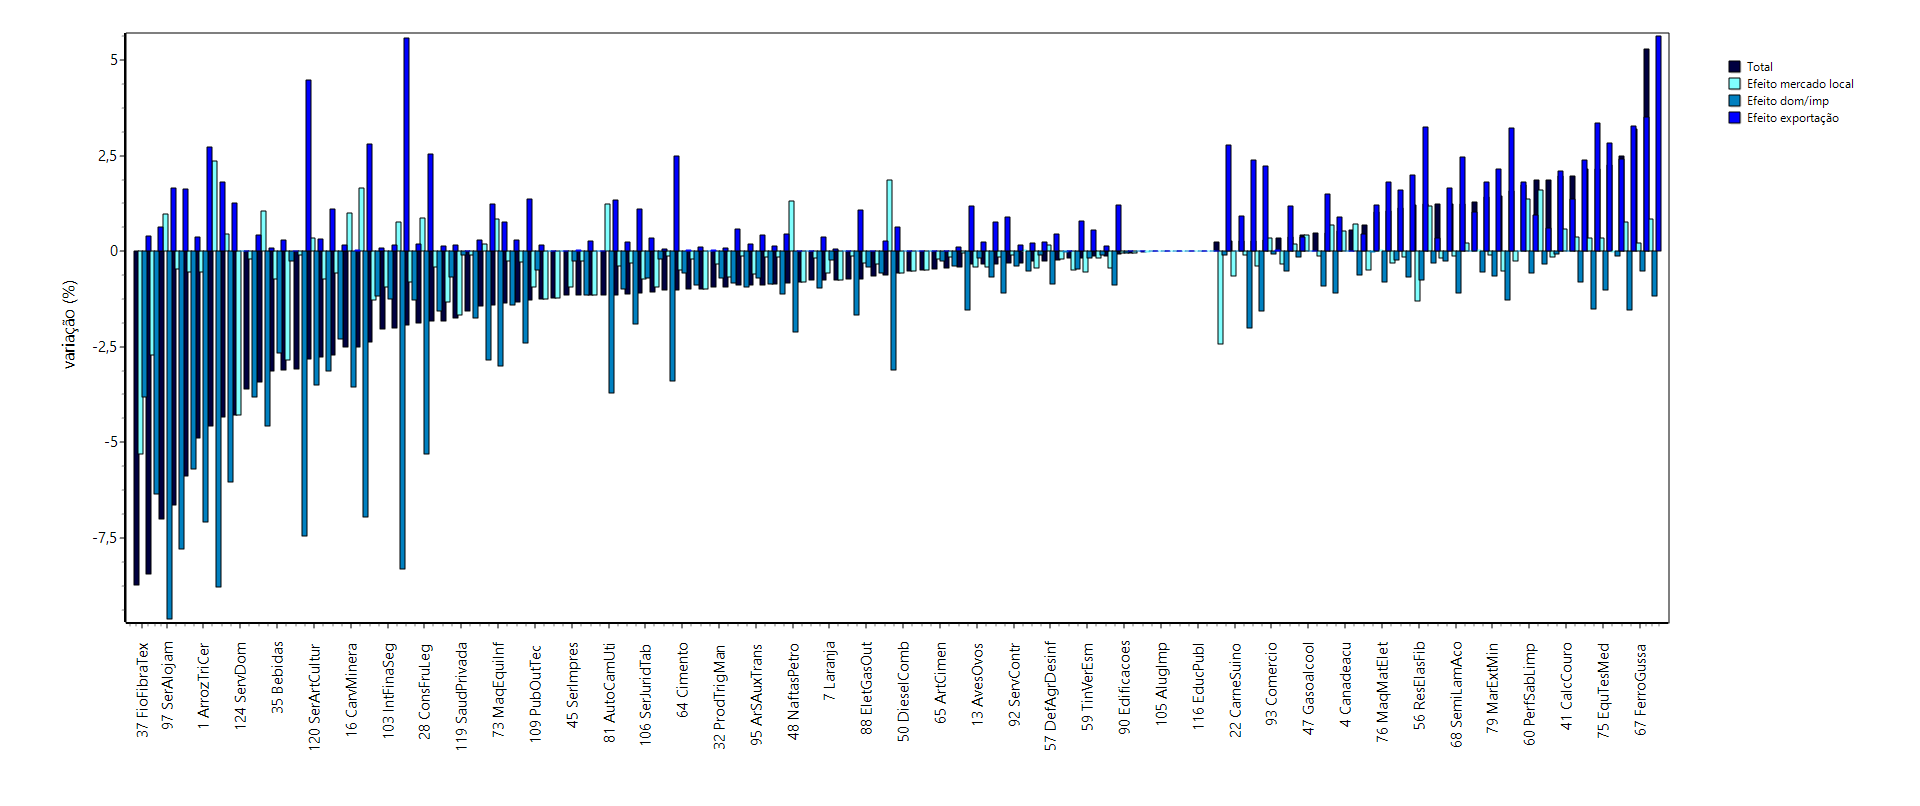
\includegraphics[width=\linewidth]{Imagens/006.ai}
		\footnotesize
		Fonte: elaboração própria (2024)
	\end{figure}
\end{landscape}


\subsection{Forma funcional} \label{subsec:forma_funcional}

Esta subseção apresenta o modelo de geração da renda familiar (\textit{Household Income Generation Model}) empregado para especificar a microssimulação comportamental utilizada neste trabalho. Baseado em \textcite{bourguignon05}, esse modelo consiste no conjunto de equações a seguir:

\begin{align}
	\Log \mathcal{w}_{mi}  &= \alpha_{g} + \beta_{g} \mathcal{x}_{mi} + \upsilon_{mi} \hspace{3cm} i = 1, \ldots, k_m \label{eq:renda} \\[0.5cm]
	IW_{mi}                &= \mathbbm{1} \left[\gamma_{g} + \delta_{g} z_{mi} + \mu_{mi} \right] \label{eq:ocm} \\[0.1cm]
	\text{Y}_{m}           &= \sum_{i = 1}^{k_{m}} \mathcal{w}_{mi} IW_{mi} + y_{0m} \label{eq:renda_familiar}
\end{align}

A equação~\eqref{eq:renda} apresenta os determinantes do salário $\mathcal{w}$ do indivíduo $\mathcal{i}$ da família $\mathcal{m}$ como função de suas características individuais, $\mathcal{x}$. O subscrito $g$ indica o segmento do mercado de trabalho\footnote{Por exemplo: gênero, idade, capital humano ou situação do domicílio.} ao qual pertence o indivíduo $\mathcal{i}$ da família $\mathcal{m}$. É válido ressaltar que  $\mathcal{w}_{mi}$ considera apenas o salário do trabalho principal.

A equação~\eqref{eq:ocm} representa a escolha ocupacional do indivíduo $\mathcal{i}$ da família $\mathcal{m}$. Todos os indivíduos são confrontados com uma escolha discreta: trabalhar ou não trabalhar. Desse modo, $IW_{mi}$ é uma variável \textit{dummy} na qual zero representa o indivíduo inativo e um, trabalhador assalariado, sendo função de suas características individuais e familiares, $z$. Isto implica que o modelo não atribui a todos os indivíduos uma escolha particular, mas dá as probabilidades individuais de estar numa condição e não na outra. Ou seja, o modelo gera uma distribuição de probabilidade sobre as duas diferentes alternativas \cite{colombo08}. Por simplicidade, assume-se aqui que todos os assalariados têm jornadas integrais de trabalho.

A equação~\eqref{eq:renda_familiar} é uma identidade contábil que define o rendimento da família $Y_m$ como a soma do salário do trabalho principal, $\mathcal{w}_{mi}$, com os rendimentos de todas as outras fontes que não o trabalho principal, $y_{0m}$. A \textit{dummy} da escolha ocupacional garante que os salários que forem somados sejam apenas dos indivíduos realmente engajados no mercado de trabalho.

Desse modo, o modelo de geração da renda familiar define o salário de uma dada família $\mathcal{m}$ como função das características observadas ($\mathcal{x_{mi}}$, $z_{mi}$) e não observadas ($\upsilon_{mi}$, $\mu_{mi}$) dos indivíduos e dos familiares. Essa função depende de dois blocos de parâmetros: 1- dos determinantes de salários ($\alpha_g$, $\beta_g$); e 2- da escolha ocupacional ($\gamma_g$, $\delta_g$), ambos para os segmentos do mercado de trabalho. Com essas informações, tem-se o modelo completo. Para este trabalho, a função $g()$ representa o segmento de habilidade dos indivíduos -- não qualificado, semi-qualificado e qualificado. Desse modo, o modelo é executado três vezes, um para cada segmento, obtendo três grupos de resultados.


\subsection{Integração com o modelo EGC}\label{subsec:integracao}

O link entre um modelo EGC e uma microssimulação se dá pela variação dos parâmetros. É a partir deles que os resultados do primeiro podem ser transmitidos para a o segundo. Ou seja, a integração macro-micro consiste em associar choques macroeconômicos e alterações em políticas simuladas no modelo EGC a partir de mudanças no conjunto de parâmetros do modelo de microssimulação.

O primeiro passo para a integração é criar a simulação de \textit{benchmarking}, necessária para se obter um conjunto inicial de parâmetros da microssimulação. A partir disso, o choque macroeconômico pauta a magnitude da variação desses parâmetros para que haja a integração entre os dois modelos. Entretanto, essa associação deve ser feita de maneira consistente. Para o modelo de microssimulação proposto nesta dissertação, deve-se garantir: 1- variações nos salários da microssimulação devem ser iguais às alterações na taxa salarial obtida com o modelo EGC; e 2- as mudanças no número de trabalhadores assalariados no modelo de microssimulação devem corresponder às observadas no modelo EGC \cite{bourguignon05, colombo08}.

Isso significa que o modelo EGC determina o nível de emprego agregado da economia e o modelo de microssimulação estima a probabilidade dos indivíduos estarem ou não alocados no mercado de trabalho, dado a variação agregada. As variáveis preditas da equação~\eqref{eq:ocm} permitem classificar os indivíduos de acordo com a probabilidade de ingresso no mercado de trabalho. A partir de uma determinada nota de corte\footnote{Utilizou-se como nota de corte a taxa de desemprego para o ano de 2015 -- equivalente a 8,9\% de acordo com o IBGE.}, decide-se quais indivíduos estarão alocados no mercado de trabalho e quais não estarão. Para os indivíduos que ficaram acima da nota de corte e, por conseguinte, foram selecionados, estima-se seus salários a partir da equação~\eqref{eq:renda}.

Seja $E_G$ o nível de emprego no segmento G e $w_G$, o salário. A notação em chapéu (\^{}) indica que é uma variável estimada a partir do modelo de geração da renda familiar. Baseado em \textcite{bourguignon05}, a consistência pode ser formalizada a partir do conjunto de restrições descritas abaixo.

\begin{align}
	E_G &= \left\langle \sum_{mi}^{3} \mathbbm{1} \left[ \hat{\gamma}_g + \hat{\delta}_g z_{mi} + \hat{\mu}_{mi} \right] \right\rangle_{G} \label{eq:emprego_ag} \\
	\mathcal{w}_G &= \left\langle \sum_{mi}^{3} \text{Exp} \left( \hat{\alpha}_g + \hat{\beta}_g x_{mi} + \hat{\upsilon}_{mi} \right) \cdot \mathbbm{1} \left[ \hat{\gamma}_g + \hat{\delta}_g z_{mi} + \hat{\mu}_{mi} \right] \right\rangle_{G} \label{eq:renda_ag}
\end{align}

A equação~\eqref{eq:emprego_ag} representa a soma do nível de emprego assalariado para cada um dos segmentos do mercado de trabalho -- neste trabalho, para as três categorias do fator trabalho: não qualificado, semi-qualificado e qualificado. A equação~\eqref{eq:renda_ag} representa a massa salarial para cada um dos segmentos do mercado de trabalho.

Supõe-se agora um choque exógeno do modelo EGC que altera as variáveis ($E_G$, $w_G$) para ($E_G^*$, $w_G^*$). Buscando garantir a consistência da integração macro-micro, deve-se encontrar um novo conjunto de parâmetros $C^*$ = ($\alpha_g^*$, $\beta_g^*$, $\gamma_g^*$, $\delta_g^*$) que mantenha a mesma validade do conjunto C = ($\alpha_g$, $\beta_g$, $\gamma_g$, $\delta_g$). 

Portanto, o link entre os modelos EGC e de geração da renda familiar é obtido através da resolução do seguinte sistema de equações:

\begin{align}
	E_G^* &= \left\langle \sum_{mi}^{3} \mathbbm{1} \left[ \hat{\gamma}_{g}^* + \hat{\delta}_{g}^* z_{mi} + \hat{\mu}_{mi} \right] \right\rangle_{G} \label{eq:emprego_ag*} \\
	\mathcal{w}_G^* &= \left\langle \sum_{mi}^{3} \text{Exp} \left( \hat{\alpha}_g^* + \hat{\beta}_g^* x_{mi} + \hat{\upsilon}_{mi} \right) \cdot \mathbbm{1} \left[ \hat{\gamma}_{g}^* + \hat{\delta}_{g}^* z_{mi} + \hat{\mu}_{mi} \right] \right\rangle_{G} \label{eq:renda_ag*}
\end{align}

Uma vez solucionado esse conjunto de equações, deve-se partir para calcular a nova renda familiar per capita, conforme indicam as equações~\eqref{eq:renda} --~\eqref{eq:renda_familiar}, usando os conjuntos $C$ e $C^*$. Desse modo, tem-se, como resultado, a probabilidade de emprego, salários estimados e renda familiar per capita estimada dos indivíduos antes do choque -- cenário benchmarking -- e após o choque -- chamado aqui de cenário integração. Com essas informações, é possível calcular as estatísticas de distribuição de renda e pobreza antes e depois do choque exógeno e avaliar os efeitos dos novos parâmetros sobre o modelo de microssimulação.


\subsection{Abordagem empírica} \label{subsec:abordagem_empirica}

Uma vez definida a forma funcional da microssimulação e o processo de integração com o modelo EGC, deve-se partir para a estimação dos parâmetros do modelo de geração da renda familiar. Para este trabalho, optou-se por utilizar a Correção de Heckman para as equações~\eqref{eq:renda} e~\eqref{eq:ocm}. Apesar de haver um viés de seleção na base de dados da microssimulação\footnote{Só é observado uma renda do trabalho principal maior ou igual a zero para os indivíduos que estão empregados no momento da pesquisa amostral. Todos os outros indivíduos, necessariamente, tem \textit{missing} como renda do trabalho.}, sabe-se que Heckman não é capaz de corrigi-lo integralmente. Entretanto, na literatura de microssimulação, utiliza-se muito essa técnica com o objetivo de apenas melhorar a acurácia dos parâmetros, através de uma correção parcial do viés, sendo amplamente vista nos trabalhos de integração \textit{top--down} \cite{bourguignon05, colombo08, cury16}.

A Correção de Heckman \cite{heckman79} é dividida em duas etapas: na primeira, executa-se o modelo de escolha discreta~\eqref{eq:ocm}, que tem o objetivo de estimar a probabilidade de ingresso no mercado de trabalho via Probit. Com seus preditores lineares, calcula-se a Inversa de Mills. As equações abaixo apresentam a especificação dessa primeira etapa.

\begin{align}
	\boldsymbol{\hat{Trab}}_{g(mi)} &= \hat{\gamma}_g + \mathbf{X}_{g(mi)} \ \boldsymbol{\hat{\beta}}_g \label{eq:step1} \\
	\boldsymbol{\Lambda}_{g(mi)}    &= \frac{\phi(x)}{1 - \Phi(x)} \label{eq:mills}
\end{align}

Na qual $\boldsymbol{\hat{Trab}}_{g(mi)}$ é uma variável \textit{dummy} de participação no mercado de trabalho e $\hat{\gamma}_g$ é o intercepto da equação. $\mathbf{X}_{g(mi)}$ é uma matriz formada pelas seguintes variáveis independentes: anos de estudo, experiência potencial e experiência potencial quadrática, renda familiar per capita, número de filhos, além de variáveis de controle para gênero, raça, situação do domicílio, unidade federativa e chefe de família.

A equação~\eqref{eq:mills} exibe o cálculo da Inversa de Mills, no qual $\phi(x)$ representa função de densidade normal padrão, e $\Phi(x)$ a função de distribuição cumulativa normal padrão. Suas informações são usadas como variável explicativa na segunda etapa da Correção para corrigir parcialmente o viés de seleção e melhorar a acurácia dos parâmetros da equação~\eqref{eq:renda}. A equação~\eqref{eq:step2} apresenta sua especificação.

\begin{align}
	\mathbf{\Log \mathcal{\hat{w}}}_{g(mi)} = \hat{\alpha}_g + \mathbf{Z}_{g(mi)} \ \boldsymbol{\hat{\beta}}_g \label{eq:step2}
\end{align}

Na qual $\mathbf{\Log \mathcal{w}}_{g(mi)}$ é o logaritmo da renda-hora do indivíduo $i$ da família $m$ e $\hat{\alpha}_g$ é o intercepto da equação. $\mathbf{Z}_{g(mi)}$ é uma matriz de variáveis explicativas que contém: anos de estudo, experiência potencial e experiência potencial quadrática, situação do domicílio, Inversa de Mills e variáveis de controle por gênero, raça, setor e unidade federativa.

Toda a estimação acima descrita foi feita utilizando o desenho amostral da base de dados. A tabela com a descrição completa de todas as variáveis independentes utilizadas na microssimulação comportamental está disponível no Apêndice~\ref{ap:a}.


\subsection{Base de dados} \label{subsec:dados_microssimulacao}

Para estimar o modelo de geração da renda familiar, optou-se por utilizar os dados \citetitle*{pnad} referente ao ano de 2015. Essa base contém informações	sobre os domicílios brasileiros, as características pessoais e socioeconômicas de seus indivíduos por setor produtivo e unidade federativa, totalizando cerca de 356.904 observações. Sua escolha se baseia na necessidade de garantir compatibilidade entre os resultados dos dois modelos utilizados neste trabalho. Ao usar a PNAD 2015 para calibrar o modelo ORANIG-BR e substanciar o modelo de geração de renda familiar, abre-se espaço para que os resultados sejam compatíveis e, por conseguinte, possam dialogar entre si.



\section{Desigualdade de renda e pobreza} \label{sec:desigualdade_pobreza}

Esta seção apresenta as ferramentas utilizadas para avaliar o comportamento da desigualdade de renda e pobreza frente ao choque exógeno simulado no modelo ORANIG-BR. Em relação a desigualdade de renda, optou-se por utilizar o índice de Gini, bastante consolidado na literatura econômica. Sobre a pobreza, decidiu-se por usar a família de métricas de pobreza FGT. As subseções abaixo apresentam esse índice, bem como a linha de pobreza necessária para seu cálculo.


\subsection{Linhas de pobreza}

Os índices FGT, bem como a grande maioria das métricas de pobreza, baseiam-se em linhas de pobreza. Pode-se defini-las como uma forma de mensurar a carência de uma determinada população, demarcando o grupo que não possui à disposição todos os recursos necessários para sobreviver. Sua função é estabelecer um critério binário que divida os indivíduos em pobres e não-pobres \cite{soares09}.

Há diversas formas de mensura-las e todas derivam de alguma compreensão sobre o que é a pobreza. A Figura~\ref{fig:linhas_pobreza} ilustra as distintas formas de linhas de pobreza. Este trabalho foca nas linhas de pobreza a partir do aspecto unidimensional da pobreza: da insuficiência de renda.

\begin{figure}[h]
	\centering
	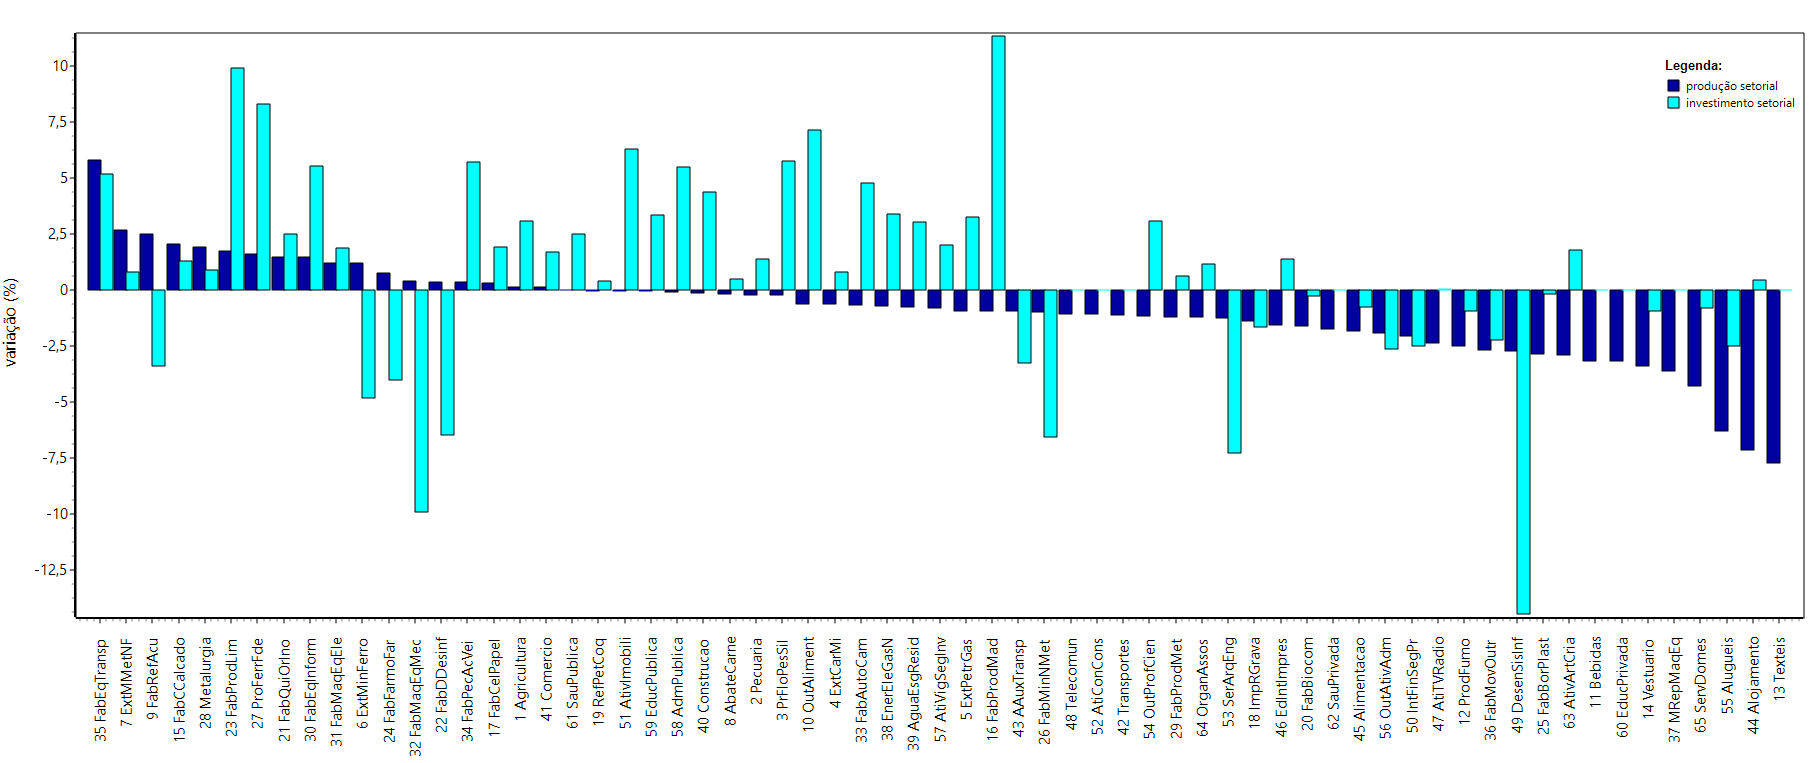
\includegraphics[width = 12cm]{Imagens/008.ai}
	\caption{Tipos de linhas de pobreza}
	\label{fig:linhas_pobreza}
	\footnotesize
	Fonte: elaboração própria (2024) a partir de \textcite{soares09}
\end{figure}

\textcite{soares09} destaca a dificuldade em obter um consenso sobre qual seria a melhor linha de pobreza. A linha absoluta tem grande dificuldade de gerar resultados comparáveis entre países, uma vez que não há um consenso sobre o que seria o mínimo necessário para que um indivíduo não seja considerado pobre. Por outro lado, as linhas relativas, por muitas vezes, acabam por confundir desigualdade com pobreza. Definitivamente uma disparidade de qualidade de vida entre indivíduos é uma evidência de desigualdade, mas não pode, necessariamente, ser considerado uma evidência de pobreza \textcite{sen83}. É preciso de mais informações sobre a renda dos indivíduos e seu acesso a serviços básicos, dentre outras variáveis, para poder afirmar se também há evidências de pobreza. Ou seja, considerações relativas sobre pobreza não podem carecer de uma âncora de natureza absoluta.

A linha de pobreza mais comumente utilizada na literatura econômica é a linha absoluta. Nessa modalidade, a mais tradicional é a criada pelo Banco Mundial, calculada através da Paridade do Poder de Compra. Em 2011, era considerado pobre os indivíduos cuja renda estivesse abaixo de US\$5,50 por dia, e os extremamente pobres, US\$1,90 por dia. Esses valores foram revisados em 2017, passando para, respectivamente, US\$6,85 e US\$2,15 por dia.

Neste trabalho, adotou-se a linha de pobreza do Banco Mundial com valores de 2011 para fins de melhor adequação ao dados utilizados da PNAD. Convertendo os valores para dezembro de 2015, as linhas de pobreza equivalem, respectivamente, a R\$126,79 e R\$367,02 por mês. 


\subsection{Índices Foster-Greer-Thorbecke}

Os índices Foster-Greer-Thorbecke são uma família de métricas de pobreza comumente utilizadas na literatura econômica para avaliar os níveis de pobreza em uma determinada sociedade. Sua fórmula geral é dada por:

\begin{align}
	\textbf{FGT}_\alpha = \frac{1}{N} \sum_{i=1}^{Q} \left( \frac{z - y_i}{z} \right)^{\alpha}
\end{align}

No qual $z$ é a linha de pobreza arbitrada, $y_i$ é o menor nível de renda do i-ésimo indivíduo, $N$ é o tamanho da população, $Q$ é a quantidade de indivíduos cuja renda está abaixo de $z$ e $\alpha$ é o parâmetro de aversão à pobreza (\textit{poverty aversion}). A fórmula geral se ramifica a partir do valor de $\alpha$. Em geral, são três subgrupos que compõem os índices FGT, listados no Quadro~\ref{quad:fgt}.

\begin{quadro}[h]
	\centering
	\begin{threeparttable}
		\caption{Descrição dos índices Foster-Greer-Thorbecke} \label{quad:fgt}
		\footnotesize
		\begin{tabular}{|llcc|}
			\hline
			\multirow{2}{*}{\textbf{Valores}} & \multicolumn{1}{c}{\multirow{2}{*}{\textbf{Fórmulas}}} & \multicolumn{2}{c|}{\textbf{Descrição}} \\ \cline{3-4} 
			 & \multicolumn{1}{c}{} & \textbf{Nome} & \textbf{Objetivo} \\ \hline
			$\alpha = 0$ & $\textbf{FGT}_0 = \frac{Q}{N}$ & \makecell{proporção de pobres \\ (\textit{headcount ratio})} & \makecell{mede a quantidade de indivíduos \\ abaixo da linha de pobreza} \\
			$\alpha = 1$ & $\textbf{FGT}_1 = \frac{1}{N} \sum_{i=1}^{Q} \left( \frac{z - y_i}{z} \right)$ & \makecell{hiato médio da pobreza \\ (\textit{poverty gap})} & \multirow{2}{*}{\makecell{mede a distância dos indivíduos \\ para alcançar a linha de pobreza$^{1}$}} \\
			$\alpha = 2$ & $\textbf{FGT}_2 = \frac{1}{N} \sum_{i=1}^{Q} \left( \frac{z - y_i}{z} \right)^{2}$ & \makecell{hiato médio da pobreza quadrática \\ (\textit{squared poverty gap})} &  \\ \hline
			\end{tabular}
		\begin{tablenotes}
			\scriptsize
			\item Fonte: elaboração própria (2024)
			\item \textit{Nota:}
			\item \hspace{0.2cm} $^{1}$por ser uma equação quadrática, o $\text{FGT}_2$ confere maior peso aos indivíduos mais pobres.
		\end{tablenotes}
	\end{threeparttable}
\end{quadro}

A decomposição da pobreza é uma das maiores vantagens dos índices FGT, permitindo uma visão mais refinada do fenômeno. Nisso, destaca-se os dois últimos índices que permitem considerar o nível de pobreza entre os mais pobres. Ou seja, a partir deles, é possível analisar a intensidade e a severidade da pobreza entre os indivíduos abaixo da linha de pobreza. Em função disso, uma mudança na distribuição de renda tem maior efeito sobre esses dois indicadores que o próprio crescimento da renda \cite{kraay04}.

Mesmo assim, o primeiro índice cumpre uma função importante na avaliação da pobreza em uma determinada sociedade. Apesar de sua simplicidade, seus resultados são sensíveis a variações absolutas da renda, sendo um bom indicador para medir crescimento da renda dos indivíduos. Nisso, ele se difere dos outros dois índices que dão maior ênfase à distribuição de renda, focando, portanto, em variações relativas da renda.


